\documentclass[12pt]{article}
\usepackage[margin=0.9in,headheight=16pt]{geometry}
\usepackage[T1]{fontenc}
\usepackage{lmodern}
\usepackage{graphicx}
\graphicspath{{../../figures/}{../figures/}{figures/}}
\usepackage{array}
\usepackage{booktabs}
\usepackage{longtable}
\usepackage{tabularx}
\usepackage{float}
\usepackage{caption}
\usepackage{amsmath}
\usepackage{amssymb}
\usepackage{tikz}
\usetikzlibrary{arrows.meta,positioning,shapes.geometric}
\usepackage{enumitem}
\usepackage{hyperref}
\usepackage{xcolor}
\usepackage{etoolbox}
\usepackage{fancyhdr}
\usepackage{titlesec}
\usepackage{setspace}

\definecolor{psidblue}{HTML}{1E3A5F}
\definecolor{psidink}{HTML}{1F2937}
\definecolor{psidmuted}{HTML}{4B5563}
\definecolor{psidline}{HTML}{D1D5DB}
\definecolor{psidpanel}{HTML}{F7FAFC}
\definecolor{psidaccent}{HTML}{E8F1FB}
\definecolor{psidgold}{HTML}{A16207}

\hypersetup{
  colorlinks=true,
  linkcolor=psidblue,
  urlcolor=psidblue,
  citecolor=psidblue,
  pdftitle={PSID Client Report},
  pdfauthor={GitHub Copilot}
}

\makeatletter
\g@addto@macro\UrlBreaks{\do\_\do\/\do\-}
\makeatother

\captionsetup{
  font=small,
  labelfont={bf,sf,color=psidblue},
  justification=raggedright,
  singlelinecheck=false
}
\captionsetup[table]{position=top}

\setlength{\parindent}{0pt}
\setlength{\parskip}{5pt}
\setlength{\tabcolsep}{3.5pt}
\setlength{\LTleft}{0pt}
\setlength{\LTright}{0pt}
\renewcommand{\arraystretch}{1.14}
\setlist[itemize]{leftmargin=1.5em, itemsep=0.2em, topsep=0.3em}
\setlist[enumerate]{leftmargin=1.6em, itemsep=0.25em, topsep=0.3em}
\setstretch{1.08}
\emergencystretch=1.5em

\newcolumntype{L}[1]{>{\raggedright\arraybackslash\hspace{0pt}}p{#1}}
\newcolumntype{C}[1]{>{\centering\arraybackslash}p{#1}}
\newcolumntype{R}[1]{>{\raggedleft\arraybackslash}p{#1}}
\newcolumntype{Y}{>{\raggedright\arraybackslash\hspace{0pt}}X}

\newcommand{\reportseries}{PSID Crisis Module Client Series}
\newcommand{\reporttitle}{Client Report}
\newcommand{\reportsubtitle}{PSID Crisis Module}
\newcommand{\reportclient}{Client Deliverable}
\newcommand{\reportversion}{April 2026}
\newcommand{\reportstatus}{Prepared for client review}
\newcommand{\reportabstract}{}
\newcommand{\reportkeywords}{}
\newcommand{\reportdoi}{\url{https://github.com/namo507/Team-PSID}}
\newcommand{\varname}[1]{\nolinkurl{#1}}
\newcommand{\filepath}[1]{\nolinkurl{#1}}

\pagestyle{fancy}
\fancyhf{}
\fancyhead[L]{\sffamily\footnotesize \reporttitle}
\fancyhead[R]{\sffamily\footnotesize \thepage}
\fancyfoot[L]{\sffamily\footnotesize \reportclient}
\fancyfoot[R]{\sffamily\footnotesize Team-PSID}

\fancypagestyle{plain}{
  \fancyhf{}
  \fancyhead[L]{\sffamily\footnotesize \reporttitle}
  \fancyhead[R]{\sffamily\footnotesize \thepage}
  \fancyfoot[L]{\sffamily\footnotesize \reportclient}
  \fancyfoot[R]{\sffamily\footnotesize Team-PSID}
}

\titleformat{\section}{\Large\bfseries\sffamily\color{psidblue}}{\thesection}{0.75em}{}
\titleformat{\subsection}{\large\bfseries\sffamily\color{psidink}}{\thesubsection}{0.65em}{}
\titleformat{\subsubsection}{\normalsize\bfseries\sffamily\color{psidink}}{\thesubsubsection}{0.5em}{}

\newsavebox{\psidboxbox}
\newenvironment{psidbox}[1]{%
  \par\medskip
  \begin{center}
  \setlength{\fboxsep}{12pt}%
  \begin{lrbox}{\psidboxbox}
  \begin{minipage}{0.94\linewidth}
  {\sffamily\bfseries\color{psidblue}#1}\par\medskip
}{%
  \end{minipage}
  \end{lrbox}
  \fcolorbox{psidline}{psidpanel}{\usebox{\psidboxbox}}
  \end{center}
  \par\medskip
}

\newcommand{\makecover}{%
  \pagenumbering{arabic}
  \thispagestyle{plain}
  {\sffamily\footnotesize\color{psidmuted}\reportseries\hfill \reportclient\par}
  \vspace{0.35cm}
  {\sffamily\bfseries\fontsize{22}{26}\selectfont \reporttitle\par}
  \vspace{0.15cm}
  {\sffamily\Large\color{psidmuted} \reportsubtitle\par}
  \vspace{0.3cm}
  {\footnotesize\color{psidmuted}\reportstatus\quad|\quad Updated: \reportversion\quad|\quad \reportdoi\par}
  \vspace{0.35cm}
  \begin{psidbox}{Abstract}
  \reportabstract
  \end{psidbox}
  \ifstrempty{\reportkeywords}{}{%
    {\sffamily\small\textbf{Keywords:} \reportkeywords\par}
    \vspace{0.2cm}
  }
  {\color{psidline}\rule{\textwidth}{0.9pt}}\par
  \vspace{0.45cm}
}

\newcommand{\psidfigure}[3][0.92]{%
  \begin{figure}[H]
  \centering
  \fcolorbox{psidline}{white}{\includegraphics[width=#1\linewidth]{#2}}
  \caption{#3}
  \end{figure}
}

\tikzset{
  flowstep/.style={
    rectangle,
    rounded corners=6pt,
    draw=psidblue,
    fill=psidpanel,
    very thick,
    align=center,
    text width=3.6cm,
    minimum height=1cm,
    font=\sffamily\small
  },
  flowwide/.style={flowstep, text width=4.4cm},
  flowresult/.style={flowstep, draw=psidgold!85!black, fill=psidaccent},
  flowarrow/.style={-{Stealth[length=3mm]}, very thick, draw=psidblue}
}

\renewcommand{\reporttitle}{Client 1: Technical Codebook}
\renewcommand{\reportsubtitle}{Refreshed PSID crisis-module workflow, scoring logic, and artifact schema}
\renewcommand{\reportclient}{Technical Deliverable}

\begin{document}

\makecover

\section{Purpose and Scope}

This technical codebook documents the refreshed PSID crisis-module workflow from the authoritative ranked source file through the final scored CSV, figures, spreadsheet, and PDF bundle. It is written to support analytic review, reproducibility, and downstream client sign-off.

\begin{psidbox}{Production status}
\begin{itemize}
\item 52 ranked historical questions in the current corpus.
\item 28 selected rows in the scored module and 26 questions in the deployable instrument.
\item 3 \texttt{Generic} rows and 49 \texttt{Specific} rows after binary thresholding.
\item 29.98 selected minutes in the scored module and 28.82 minutes in the deployable instrument.
\item The 28-to-26 change comes from excluding \varname{SPC_AGE_YEARS} and \varname{SPC_DESCRIBE_SEX_GENDER} from routine field administration while retaining them for traceability.
\end{itemize}
\end{psidbox}

\section{Headline Benchmark Summary}

\begin{table}[H]
\centering
\small
\begin{tabularx}{\textwidth}{L{0.22\textwidth} R{0.10\textwidth} Y Y}
\toprule
Metric & Value & Calculation / rule & Why it is used and the assumption behind it \\
\midrule
Total ranked questions & 52 & $\operatorname{count}(\text{all rows}) = 52$ & Starting analytic universe; assumes the integrated source file is the authoritative corpus for each refresh. \\
Selected scored questions & 28 & $\operatorname{count}(\texttt{selected\_for\_module}=\texttt{True}) = 28$ & Defines the scored review package under the fixed 30-minute module cap. \\
Deployable questions & 26 & $28 - 2 = 26$ after removing selected demographic-only traceability rows & Produces the live instrument; assumes demographic context can be collected elsewhere or only when routing requires it. \\
Selected scored minutes & 29.98 & $\sum \text{minutes over the 28 selected rows} = 29.98$ & Confirms the scored module stays within the client's review budget. \\
Deployable minutes & 28.82 & $29.98 - 0.35 - 0.817 = 28.813 \approx 28.82$ & Paper-length estimate for the field instrument after age and sex/gender are removed from routine administration. \\
Full corpus minutes & 68.60 & $\sum \text{minutes over all 52 rows} = 68.60$ & Shows why a selection layer is required; assumes every row would otherwise be asked. \\
Generic rows & 3 & $\operatorname{count}(\text{ri\_threshold\_score} \geq 0.70) = 3$ after normalization & Keeps the universal portable core intentionally small; assumes the binary split should surface only the strongest cross-crisis items. \\
Specific rows & 49 & $52 - 3 = 49$ & Keeps direct crisis-detail items in the context-sensitive bank. \\
Average $R_i$ & 2.201 & $\operatorname{mean}(R_i) = 2.201$ & Benchmark statistic only; not itself a cutoff rule. \\
Maximum $R_i$ & 5.667 & $\max(R_i) = 5.667$ & Upper bound for min-max normalization in the current refresh. \\
Average $P_i$ & 2.561 & $\operatorname{mean}(P_i) = 2.561$ & Tracks distinctiveness-adjusted priority across the corpus. \\
Maximum $P_i$ & 7.860 & $\max(P_i) = 7.860$ & Shows the ceiling after rarity, construct, portability, and redundancy adjustments. \\
\bottomrule
\end{tabularx}
\caption{Current benchmark summary used by the maintained client package.}
\end{table}

\section{Why 28 Scored Rows Become 26 Deployable Questions}

\begin{table}[H]
\centering
\footnotesize
\begin{tabularx}{\textwidth}{L{0.20\textwidth} R{0.08\textwidth} R{0.10\textwidth} Y Y}
\toprule
Stage & Rows & Minutes & Calculation / rule & Why it is retained or removed \\
\midrule
Full ranked corpus & 52 & 68.60 & Count of all rows in the integrated source; minutes are summed across the corpus & Starting point for ranking, diagnostics, and documentation. \\
Scored module & 28 & 29.98 & Count of selected rows after ranking and time-budget filtering & Preserves the full analytic shortlist, including traceability fields. \\
Selected demographic traceability rows & 2 & 1.17 & \varname{SPC_AGE_YEARS} $(0.35)$ + \varname{SPC_DESCRIBE_SEX_GENDER} $(0.817)$ & Useful for framing and optional routing, but comparatively weak as direct crisis-impact questions. \\
Deployable instrument & 26 & 28.82 & $28 - 2 = 26$ and $29.98 - 1.167 = 28.813 \approx 28.82$ & Final asked instrument prioritizes direct crisis-impact content instead of forcing demographic context into every interview. \\
\bottomrule
\end{tabularx}
\caption{The change from 28 scored rows to 26 deployable questions is a deployment optimization, not a re-ranking of the corpus.}
\end{table}

\begin{psidbox}{Interpretation}
The model still selects 28 rows as the best analytic bundle under the budget. The deployable version removes only the two demographic-only rows because they are better treated as traceability or conditional-routing variables than as routine crisis-module questions.
\end{psidbox}

\section{Figures and Visual Diagnostics}

\psidfigure{fig_top_ranked_questions.png}{Top-ranked questions from the refreshed corpus.}
\psidfigure{fig_utility_vs_burden.png}{Utility-versus-burden view used to inspect signal efficiency.}
\psidfigure{fig_construct_heatmap.png}{Construct coverage heatmap for the refreshed item bank.}

\section{End-to-End Workflow Pipeline}

\begin{figure}[H]
\centering
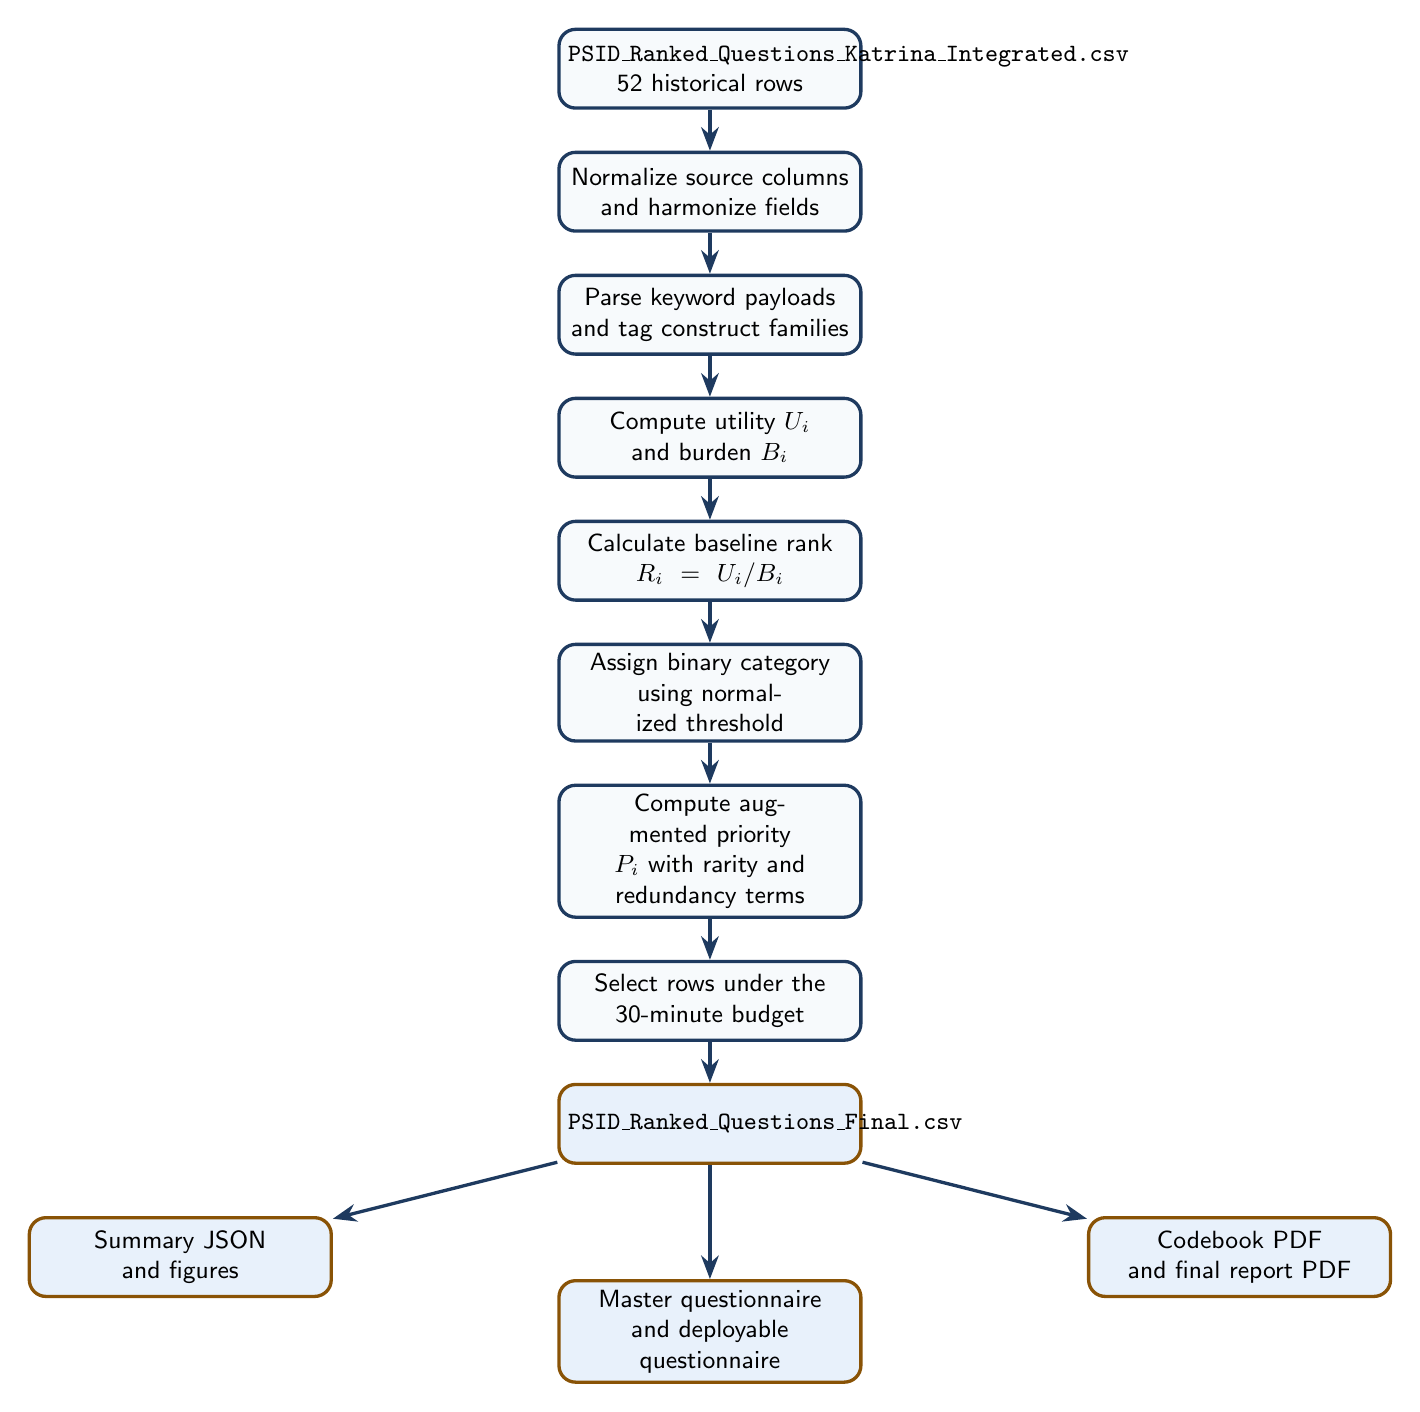
\begin{tikzpicture}[node distance=0.52cm]
\node[flowstep] (a) {\texttt{PSID\_Ranked\_Questions\_Katrina\_Integrated.csv}\\52 historical rows};
\node[flowstep, below=of a] (b) {Normalize source columns\\and harmonize fields};
\node[flowstep, below=of b] (c) {Parse keyword payloads\\and tag construct families};
\node[flowstep, below=of c] (d) {Compute utility $U_i$\\and burden $B_i$};
\node[flowstep, below=of d] (e) {Calculate baseline rank\\$R_i = U_i / B_i$};
\node[flowstep, below=of e] (f) {Assign binary category\\using normalized threshold};
\node[flowstep, below=of f] (g) {Compute augmented priority\\$P_i$ with rarity and redundancy terms};
\node[flowstep, below=of g] (h) {Select rows under the\\30-minute budget};
\node[flowresult, below=of h] (i) {\texttt{PSID\_Ranked\_Questions\_Final.csv}};
\node[flowresult, below left=0.65cm and 2.85cm of i] (j) {Summary JSON\\and figures};
\node[flowresult, below=1.45cm of i] (k) {Master questionnaire\\and deployable questionnaire};
\node[flowresult, below right=0.65cm and 2.85cm of i] (l) {Codebook PDF\\and final report PDF};
\draw[flowarrow] (a) -- (b);
\draw[flowarrow] (b) -- (c);
\draw[flowarrow] (c) -- (d);
\draw[flowarrow] (d) -- (e);
\draw[flowarrow] (e) -- (f);
\draw[flowarrow] (f) -- (g);
\draw[flowarrow] (g) -- (h);
\draw[flowarrow] (h) -- (i);
\draw[flowarrow] (i) -- (j);
\draw[flowarrow] (i) -- (k);
\draw[flowarrow] (i) -- (l);
\end{tikzpicture}
\caption{Production workflow from the raw integrated source to the maintained client package.}
\end{figure}

\section{Optimization Strategy Change}

\begin{table}[H]
\centering
\small
\begin{tabularx}{\textwidth}{L{0.19\textwidth} Y Y Y}
\toprule
Dimension & Legacy architecture view & Current production view & Why the change matters \\
\midrule
Client-facing categories & Legacy architecture used 7 Generic Core rows, 1 Financial Crisis row, and 20 Pandemic / Disaster rows inside the same 28-row shortlist & Current production uses 3 Generic and 25 Specific rows in the scored module, with 3 Generic and 23 crisis-specific rows in the deployable instrument & The client narrative is now binary and easier to defend; the universal core is intentionally narrower. \\
Financial representation & Finance appeared as its own visible toggle label & Financial rows now compete inside Specific and are moderated by redundancy penalties & Near-duplicate earnings and aid items no longer create the impression of a separate finance-only module. \\
Deployment target & The scored shortlist was closer to the field-facing view & The 28-row scored file is retained for auditability, while the 26-row deployable file is used for routine administration & Separates analytic traceability from operational burden. \\
Optimization levers & Score plus legacy toggle structure & Score plus portability bonus, construct coverage, redundancy control, and documentation-backed wording replacements & The instrument is optimized for an always-on, cross-crisis deployment setting rather than only for archival structure. \\
Routing refinement & Category labels described broad source-specific routing & Generic answers and crisis identification activate one relevant specific block instead of treating the full package as a single interview path & Respondent answers now reduce effective burden in live administration without overwriting the stored row scores. \\
\bottomrule
\end{tabularx}
\caption{From the legacy multi-label architecture to the current production optimization strategy.}
\end{table}

\section{Respondent-Answer Refinement and Optimization}

\begin{table}[H]
\centering
\small
\begin{tabularx}{\textwidth}{L{0.22\textwidth} Y Y Y}
\toprule
Refinement input & Quantitative effect & Why it is used & Working assumption \\
\midrule
Universal Generic answers and crisis identification & Effective live path becomes the 3-item Generic core plus one specific block; for example pandemic path minutes are $1.40 + 2.92 = 4.32$ instead of all 26 deployable items & Cuts unnecessary burden and keeps the interview aligned to the active crisis context & One dominant crisis context is active in a given administration. \\
Selected demographic answers & Removing \varname{SPC_AGE_YEARS} $(0.35)$ and \varname{SPC_DESCRIBE_SEX_GENDER} $(0.817)$ lowers the base deployable length by $1.167$ minutes & Preserves traceability without forcing low-yield context items into every interview & Demographic information can be captured elsewhere or only when routing requires it. \\
Historical respondent distributions & Shutdown coping, stimulus uptake, and pandemic response patterns support keeping Government Aid and Financial Coping constructs salient in the selected bank & Grounds construct weights and wording choices in observed crisis behavior rather than only lexical similarity & Historical respondent patterns are informative for future crisis-module design. \\
Feed-forward respondent state & Prior-wave status, identity, address, and eligibility can refine universes or wording windows, but do not overwrite stored $U_i$, $B_i$, $R_i$, or $P_i$ values & Distinguishes static ranking from live survey routing & Prior-wave metadata is available when the module is deployed longitudinally. \\
\bottomrule
\end{tabularx}
\caption{Respondent data influences deployment and construct emphasis even when the stored row scores remain fixed.}
\end{table}

The respondent-data evidence used for refinement is substantive rather than cosmetic. In the reference evidence, 70.6\% of shutdown-affected families cut spending, 28.3\% used food banks, and pandemic response data show strong heterogeneity in vaccination and stimulus behavior. Those patterns explain why coping, aid, earnings-loss, and health-response items remain prominent after redundant variants are pruned.

\section{Files and Roles}

\begin{table}[H]
\centering
\small
\begin{tabularx}{\textwidth}{L{0.27\textwidth} L{0.22\textwidth} Y}
\toprule
File & Role & Why it matters \\
\midrule
\texttt{data/PSID\_Ranked\_Questions\_Katrina\_Integrated.csv} & Raw integrated source bank & Starting point for every production rebuild. \\
\texttt{PSID\_NLP\_Crisis\_Module\_Structure.py} & Shared scoring helpers & Holds constants, keyword parsing, burden logic, threshold helpers, and selection utilities. \\
\texttt{generate\_psid\_artifacts.py} & Production rebuild engine & Writes the final scored CSV, summary JSON, dashboard payload, and figures. \\
\texttt{data/PSID\_Ranked\_Questions\_Final.csv} & Authoritative scored output & Main ranked table used by the notebook and client deliverables. \\
\texttt{PSID\_NLP\_Crisis\_Module\_Final.ipynb} & Validation notebook & Recomputes the workflow and verifies the persisted artifact bundle. \\
\texttt{generate\_client\_documents.py} & Client-package renderer & Builds the spreadsheet and PDFs from the scored CSV and summary JSON. \\
\texttt{data/psid\_artifact\_summary.json} & Metric bundle & Stores benchmark counts and score summaries for the latest run. \\
\bottomrule
\end{tabularx}
\caption{Files that drive the maintained workflow and client package.}
\end{table}

\section{Core Scoring Logic}

\subsection{Utility, burden, and baseline rank}

The baseline score is driven by question utility relative to response burden.

\begin{psidbox}{Core formulae}
\begin{align*}
U_i &= \sum \text{keyword weights} \\
B_i &= \max(0.10 \times \text{word\_count} + 0.20 \times \text{complexity}, 0.1) \\
R_i &= \frac{U_i}{B_i}
\end{align*}

\begin{itemize}
\item $U_i$ rewards crisis-relevant content signaled by tagged keywords.
\item $B_i$ penalizes long or complex wording.
\item $R_i$ ranks items that carry more signal per unit of burden.
\end{itemize}
\end{psidbox}

\subsection{Binary category assignment}

The client requirement was a binary rule based on $R_i$, but the raw score is not naturally bounded in $[0, 1]$. The production pipeline therefore applies the cutoff to a min-max normalized score.

\begin{psidbox}{Operational threshold rule}
\begin{align*}
\text{ri\_threshold\_score} &= \frac{R_i - \min(R_i)}{\max(R_i) - \min(R_i)} \\
\text{Generic} &\iff \text{ri\_threshold\_score} \geq 0.70 \\
\text{Specific} &\iff \text{ri\_threshold\_score} < 0.70
\end{align*}
\end{psidbox}

\subsection{Augmented priority score}

The final prioritization score preserves $R_i$ while rewarding breadth and distinctiveness.

\begin{psidbox}{Priority adjustment}
\begin{align*}
\text{augmented\_utility} &= U_i \times \bigl(1 + 0.32 \times \text{idf\_scaled} + 0.24 \times \text{construct\_scaled} \\
&\qquad\qquad + 0.12 \times \text{richness\_scaled} + \text{portability\_bonus}\bigr) \\
P_i &= \frac{\text{augmented\_utility}}{B_i \times (1 + 0.65 \times \text{redundancy\_scaled})}
\end{align*}

\begin{itemize}
\item $P_i$ helps separate distinct, portable items from repetitive variants.
\item The shortlist is still bounded by the time budget, not only by raw rank.
\end{itemize}
\end{psidbox}

\subsection{Why each quantitative field exists}

\begin{table}[H]
\centering
\small
\begin{tabularx}{\textwidth}{L{0.16\textwidth} Y Y Y}
\toprule
Quantity & Calculation & Why it is used & Assumption \\
\midrule
$U_i$ & $\sum \text{keyword weights}$ & Captures substantive crisis relevance signaled by tagged constructs & Tagged keywords are a defensible proxy for item content. \\
$B_i$ & $\max(0.10 \times \text{word\_count} + 0.20 \times \text{complexity}, 0.1)$ & Penalizes long or cognitively difficult wording & Administration burden grows approximately with length and complexity. \\
$R_i$ & $U_i / B_i$ & Measures signal per unit of burden & High-value questions should be informative relative to the time they consume. \\
\texttt{ri\_threshold\_score} & $(R_i - \min R_i)/(\max R_i - \min R_i)$ & Makes the client's $0.70$ threshold meaningful on an otherwise unbounded score & The current corpus minimum and maximum are authoritative for the refresh. \\
augmented utility & $U_i \times (1 + 0.32\,\text{idf\_scaled} + 0.24\,\text{construct\_scaled} + 0.12\,\text{richness\_scaled} + \text{portability\_bonus})$ & Rewards rarity, coverage breadth, and wording portability before redundancy is applied & Distinct and portable content adds more deployment value than repeated variants. \\
$P_i$ & $\text{augmented\_utility} / [B_i \times (1 + 0.65\,\text{redundancy\_scaled})]$ & Breaks ties among similar $R_i$ values by down-weighting repetitive items & Short modules should prefer distinct questions over clusters of near-duplicates. \\
minutes & $(\text{word\_count} \times 7)/60$ & Operational time field used in the budget and instrument assembly & Oral administration takes about 7 seconds per word on average. \\
selected rows & Time-budget filter after ranking & Defines the scored module for review and traceability & The 30-minute scored-module cap is fixed for the current package. \\
deployable rows & Selected rows minus demographic-only traceability rows & Defines the field instrument & Demographic context is not part of the core crisis ask unless routing requires it. \\
\bottomrule
\end{tabularx}
\caption{Formula, purpose, and assumption guide for the main quantitative fields.}
\end{table}

\section{Worked Calculation Example}

Example question: \texttt{GEN\_LOSE\_EARNINGS\_PANDEMIC}\\
Recommended wording: \emph{Did you lose earnings because of the pandemic?}

\begin{table}[H]
\centering
\small
\begin{tabularx}{\textwidth}{L{0.16\textwidth} R{0.10\textwidth} Y Y}
\toprule
Field & Value & Calculation & Why it is used / assumption \\
\midrule
$U_i$ & 3.400 & $0.80 + 0.80 + 0.90 + 0.90$ & Utility aggregates the matched crisis-signal weights; assumes the tagged keywords capture the substantive content of the item. \\
word count & 6 & Counted from deployable wording & Used in both burden and time estimates; assumes the cleaned wording is the administered string. \\
complexity & 0.0 & Precomputed complexity field & Prevents an additional burden penalty; assumes the wording is direct and does not require extra respondent processing. \\
$B_i$ & 0.600 & $\max(0.10 \times 6 + 0.20 \times 0.0, 0.1)$ & Converts wording cost into a penalty term; assumes the burden constants remain fixed design choices. \\
$R_i$ & 5.667 & $3.40 / 0.60$ & Measures signal efficiency; assumes high-value universal questions should deliver strong utility per unit of burden. \\
threshold score & 1.000 & $(5.667 - 0.818) / (5.667 - 0.818)$ & Supports the binary split; assumes the current refresh min and max are the correct normalization anchors. \\
Final category & Generic & $1.000 \geq 0.70$ & Places the item in the universal core; assumes the client wants only the top portable items to be Generic. \\
$P_i$ & 7.860 & Value computed after rarity, construct, richness, portability, and redundancy scaling & Separates this item from similar crisis questions; assumes distinct portable items deserve priority in a short module. \\
minutes & 0.70 & $(6 \times 7) / 60$ & Feeds the time budget; assumes oral administration averages 7 seconds per word. \\
\bottomrule
\end{tabularx}
\caption{Worked example for one of the highest-value Generic items.}
\end{table}

\section{Threshold Diagnostics}

\begin{table}[H]
\centering
\begin{tabularx}{\textwidth}{L{0.36\textwidth} R{0.12\textwidth} Y}
\toprule
Threshold diagnostic & Value & Calculation / implication \\
\midrule
Minimum raw $R_i$ & 0.818 & $\min(R_i)$ across the 52-row corpus. \\
Maximum raw $R_i$ & 5.667 & $\max(R_i)$ across the 52-row corpus. \\
Rows with raw $R_i \geq 0.70$ & 52 of 52 & Shows that a direct raw cutoff would classify every row as Generic. \\
Rows with normalized threshold score $\geq 0.70$ & 3 of 52 & Final Generic count after min-max normalization. \\
\bottomrule
\end{tabularx}
\caption{Why normalized thresholding is required for a meaningful binary split.}
\end{table}

\begin{psidbox}{Interpretation}
Raw $R_i \geq 0.70$ would classify every row as \texttt{Generic}. Normalized thresholding preserves the requested cutoff while still creating a real binary split between portable high-signal items and context-dependent items.
\end{psidbox}

\section{Construct Coverage and Interaction Notes}

\subsection{Selected construct coverage}

\begin{table}[H]
\centering
\begin{tabularx}{0.58\textwidth}{L{0.38\textwidth} R{0.10\textwidth}}
\toprule
Construct & Selected questions \\
\midrule
Trauma / Health & 15 \\
Employment & 7 \\
Housing / Shelter & 6 \\
Government Aid & 5 \\
Economic / Income & 4 \\
Financial Coping & 2 \\
Demographics & 2 \\
\bottomrule
\end{tabularx}
\caption{Construct coverage in the selected scored module.}
\end{table}

\subsection{Demographic interaction summary}

\begin{table}[H]
\centering
\begin{tabularx}{0.78\textwidth}{L{0.34\textwidth} R{0.10\textwidth} R{0.12\textwidth} R{0.12\textwidth}}
\toprule
Group & Rows & Average $R_i$ & Average $P_i$ \\
\midrule
Demographics only & 3 & 1.354 & 2.189 \\
Non-demographic crisis items & 49 & 2.253 & 2.584 \\
\bottomrule
\end{tabularx}
\caption{Demographic-only rows versus direct crisis-impact rows.}
\end{table}

\begin{psidbox}{Interpretation}
Demographic-only items remain useful for traceability and module framing, but they carry less direct crisis signal than employment, housing, aid, trauma, and economic disruption items. That is why the final deployable questionnaire excludes demographics even though the master review file retains them.
\end{psidbox}

\section{Output Schema}

\begin{table}[H]
\centering
\small
\begin{tabularx}{\textwidth}{L{0.28\textwidth} Y}
\toprule
Field & Meaning \\
\midrule
\texttt{variable\_name} & Stable identifier used across the CSV, spreadsheet, and PDFs. \\
\texttt{question\_text} & Historical source wording. \\
\texttt{recommended\_wording} & Clean deployable wording. \\
\texttt{source} & Historical module source. \\
\texttt{toggle\_category} & Final binary category: \texttt{Generic} or \texttt{Specific}. \\
\texttt{historical\_toggle\_category} & Legacy category kept for traceability. \\
\texttt{U\_i}, \texttt{B\_i}, \texttt{R\_i} & Utility, burden, and baseline rank. \\
\texttt{ri\_threshold\_score} & Normalized rank used for binary categorization. \\
\texttt{P\_i} & Enhanced priority score. \\
\texttt{selected\_for\_module} & Final selection flag under the time cap. \\
\texttt{minutes} & Estimated administration time. \\
\texttt{constructs} & Tagged construct families. \\
\bottomrule
\end{tabularx}
\caption{Key fields preserved in the authoritative scored dataset.}
\end{table}

\section{Deliverables Produced From the Same Dataset}

\begin{table}[H]
\centering
\begin{tabularx}{\textwidth}{L{0.28\textwidth} L{0.18\textwidth} Y}
\toprule
Deliverable & Audience & Purpose \\
\midrule
\filepath{deliverables/Master_Questionnaire.xlsx} & Internal review & Full 52-row review sheet with categories, wording, and scores. \\
\filepath{deliverables/Deployable_Questionnaire.pdf} & Survey deployment & Final question text without demographic rows. \\
\filepath{deliverables/Codebook.pdf} & Technical review & Rendered technical codebook. \\
\filepath{deliverables/Final_Report.pdf} & Stakeholder review & Narrative summary of results and interpretation. \\
\filepath{deliverables/Client_1_Technical_Codebook.pdf} & Client circulation & LaTeX report version of this technical codebook. \\
\bottomrule
\end{tabularx}
\caption{Client-facing and internal deliverables generated from the same scored dataset.}
\end{table}

\section{Refresh Procedure}

Use this order whenever the client package is refreshed:

\begin{enumerate}
\item Rebuild scored artifacts via \texttt{build\_all()} in \texttt{generate\_psid\_artifacts.py}.
\item Validate notebook outputs in \texttt{PSID\_NLP\_Crisis\_Module\_Final.ipynb}.
\item Regenerate spreadsheet and PDFs through \texttt{generate\_client\_documents.py}.
\item Rebuild the client-facing LaTeX reports through \texttt{docs/latex/build\_client\_reports.sh}.
\item Confirm that metrics, figures, tables, and deliverable paths remain aligned.
\end{enumerate}

That sequence keeps the scored CSV, the notebook, the figures, the packaged PDFs, and the presentation-ready report files synchronized.

\end{document}